%-------------------------
% Resume in Latex
% Author : Pedro Lara
% Based on: Wilmer Gonzalez repo
% License : MIT
%------------------------

\documentclass[letterpaper,11pt]{article}

\usepackage{latexsym}
\usepackage[empty]{fullpage}
\usepackage{titlesec}
\usepackage{marvosym}
\usepackage[usenames,dvipsnames]{color}
\usepackage{verbatim}
\usepackage{enumitem}
\usepackage[hidelinks]{hyperref}
\usepackage{fancyhdr}
\usepackage[english]{babel}
\usepackage{tabularx}
\usepackage{graphicx}
\usepackage[document]{ragged2e}

% Page coloring, fonts, and logos
\usepackage{pagecolor}
\usepackage{lato}
\renewcommand{\familydefault}{\sfdefault}
\usepackage{fontawesome}
% ---

\pagestyle{fancy}
\fancyhf{} % clear all header and footer fields
\fancyfoot{}
\renewcommand{\headrulewidth}{0pt}
\renewcommand{\footrulewidth}{0pt}

% Adjust margins
\addtolength{\oddsidemargin}{-0.5in}
\addtolength{\evensidemargin}{-0.5in}
\addtolength{\textwidth}{1in}
\addtolength{\topmargin}{-.5in}
\addtolength{\textheight}{1.0in}
\urlstyle{same}
\raggedbottom
\raggedright
\setlength{\tabcolsep}{0in}
% ---

% Sections formatting
\titleformat{\section}{
  \vspace{-4pt}\scshape\raggedright\large
}{}{0em}{}[\color{black}\titlerule \vspace{-5pt}]
% ---

% Custom commands
\newcommand{\resumeItem}[1]{%2
  \item\small{
    %\textbf{#1}
    #1
    %{: #2 \vspace{-2pt}}
  }
}

\newcommand{\resumeSubheading}[4]{
  \vspace{8pt}\item%-1
    \begin{tabular*}{0.97\textwidth}[t]{l@{\extracolsep{\fill}}r}
      \textbf{#1} & #2 \\
      \textit{\small#3} & \textit{\small #4} \\
    \end{tabular*}\vspace{-5pt}
}
\newcommand{\resumeSubSubheading}[2]{
    \vspace{1pt}
    \begin{tabular*}{0.97\textwidth}{l@{\extracolsep{\fill}}r}
      \textit{\small#1} & \textit{\small #2} \\
    \end{tabular*}\vspace{-5pt}
}
\newcommand{\resumeSubItem}[2]{\resumeItem{#1}{#2}\vspace{-4pt}}
\renewcommand{\labelitemii}{$\circ$}
\newcommand{\resumeSubHeadingListStart}{\begin{itemize}[leftmargin=*]}
\newcommand{\resumeSubHeadingListEnd}{\end{itemize}}
\newcommand{\resumeItemListStart}{\begin{itemize}}
\newcommand{\resumeItemListEnd}{\end{itemize}\vspace{-5pt}}

\newcommand{\resumeTech}[2]{
 \textbf{#1:} #2
}

% COLOR THEMES SELECTION

%For Light theme un-comment this and comment the Dark theme section below
%\colorlet{urlcolor}{blue}
%\newcommand{\otherThemeRef}{\href{https://github.com/pedrolarben/resume/raw/master/pedro_lara_dark.pdf}{Get dark theme}}
%\newcommand{\latestVersion}{\href{https://github.com/pedrolarben/resume/raw/master/pedro_lara_light.pdf}{Get latest version \faicon{refresh}}}
%\newcommand*{\researchgatesocialsymbol}  {
\includegraphics[width=1em]{img/RG-light.png}~}

%\begin{document}
% ---

% For Dark theme un-comment this and comment the Light theme section above
\colorlet{textcolor}{white!80!gray}
\colorlet{backgroundcolor}{black!30!gray}
\colorlet{urlcolor}{blue!25!white}
\AtBeginDocument{\color{textcolor}}
\newcommand{\otherThemeRef}{\href{https://github.com/pedrolarben/resume/raw/master/pedro_lara_light.pdf}{Get light theme}}
\newcommand{\latestVersion}{\href{https://github.com/pedrolarben/resume/raw/master/pedro_lara_dark.pdf}{Get latest version 
\faicon{refresh}}}
\newcommand*{\researchgatesocialsymbol}  {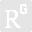
\includegraphics[width=1em]{img/RG-dark.png}~}
%
 \begin{document}
 \pagecolor{backgroundcolor}
% ---

% HEADING
\begin{tabular*}{\textwidth}{l@{\extracolsep{\fill}}r}
  \textbf{\href{https://www.pedrolarben.com}{\LARGE Pedro Lara-Benítez}} &  \\
  {{\Large Machine Learning Researcher}} &  \href{https://github.com/pedrolarben}{ \faicon{github} \color{urlcolor} pedrolarben} \\
  \href{mailto:pedrolarabenitez@gmail.com}{pedrolarabenitez@gmail.com} &  \href{https://www.linkedin.com/in/pedrolarben }{ \faicon{linkedin} \color{urlcolor} }  \href{https://scholar.google.com/citations?user=vrWKUgcAAAAJ&hl }{ \faicon{graduation-cap} \color{urlcolor} } 
  \href{https://www.researchgate.net/profile/Pedro_Lara-Benitez }{ \researchgatesocialsymbol \color{urlcolor} } \\
  \href{tel:+447895284760}{07895 284760} \hspace{0.5em} London, UK &  \faicon{code} Python, Java, C, R\\
  \textsl{\small \latestVersion} & \textsl{\small \otherThemeRef}
\end{tabular*}
% ---
\vspace{-2em}
\section*{}
\justifying
Research-focused professional with strong programming and mathematical skills in algebra and statistics. Hands-on experience providing valuable insights via data analytics and advanced data-driven methods. Proven success developing high quality code with detailed documentation to support reproducible research. Passionate about core machine learning principles, data sciences, deep learning, engineering, and research. Track record of conducting cutting-edge research on distributed artificial intelligence to develop state-of-the-art solutions for real-world problems.

% EXPERIENCE
\section{Experience}
  \resumeSubHeadingListStart
    \resumeSubheading
      {University of Seville}{Spain}
      {Machine Learning Researcher}{October 2018 - Present}
      \resumeItemListStart
      \resumeItem{
      Carry out experiments regarding deep learning, interpret results, and produce a written paper with conclusions of study.}
      \resumeItem{Demonstrate expertise in the state-of-art techniques of the field..}
      \resumeItem{Reviewed and published papers while acting as a PhD student.}
      \resumeItemListEnd
      \resumeTech{Technologies}{Python, Tensorflow, Keras, Pytorch, Sklearn, Matplotlib, AWS, Latex.}\\
      \resumeTech{Theory}{Deep Learning, Time series forecasting, Online learning, Data stream, Computer vision and Object detection.}

%\resumeSubheading
%      {\textit{Additional Experience}}{Spain}
%      {Freelance Software Developer}{2017 - 2019}
%      \resumeItemListStart
%      \resumeItem{Android App for MSIG Smart Management.}
%      \resumeItem{Patients management web information system for BBA Medical Centre.}
%      \resumeItemListEnd

\resumeSubHeadingListEnd
% ---
% PROGRAMMING SKILLS
\section{Other programming tools}
  \resumeSubHeadingListStart
  \resumeSubItem{\textbf{Cloud services:} AWS and Azure for training Deep Learning models.}
  
  \resumeSubItem{\textbf{Deep learning frameworks:} Keras, Tensorflow, Pytorch.}
  
  \resumeSubItem{\textbf{Python:} numpy, xgboost, sci-kit, pandas, river, matplotlib, flask...}
  
  \resumeSubItem{\textbf{Other technologies:} Git, docker, databases, linux, OOP<<<<<<<<.}
  
  \resumeSubHeadingListEnd

% EDUCATION
\section{Education}
  \resumeSubHeadingListStart
    \resumeSubheading
      {University of Seville}{Seville, Spain}
      {PhD in Computer Science - Machine Learning }{Sept. 2019 -- Present}
      \resumeItemListStart
      \resumeItem{Researching about data science, machine learning and artificial intelligence. Mainly focused on deep learning, time series analysis, data stream mining and object detection.}
      \resumeItemListEnd
    \resumeSubheading
      {University of Seville}{Seville, Spain}
      {M.Sc in Software Engineering: Cloud, Data Science \& IT Service Management - 9.3/10}{Sept. 2018 -- Jun. 2019}
      \resumeItemListStart
      \resumeItem{Took selective courses on: Data Engineering, Machine Learning, Data visualisation techniques, Analysis of unstructured information, Big Data, Data Science.}
      \resumeItem{(Thesis title) Asynchronous framework for the application of Deep Learning to streaming data.}
      \resumeItemListEnd
    \resumeSubheading
      {Middlesex University}{London, UK}
      {[Erasmus year abroad] B.Sc in Computer Science}{Sept. 2017 -- Jun. 2018}
      \resumeItemListStart
      \resumeItem{Took selective courses on: Open Source Software, Quantum Information Theory and Artificial Intelligence.}
      \resumeItemListEnd
    \resumeSubheading
      {University of Seville}{Seville, Spain}
      {B.Sc in Computer Science - Software Engineering - 8.5/10}{Sept. 2014 -- Jun. 2018}
      \resumeItemListStart
      \resumeItem{Took courses such as: Statistics, Analysis and Design of Data structures and Algorithms, Signal processing or Artificial Intelligence.}
      \resumeItem{(Thesis title) Biomedical data analysis with deep learning.}
      \resumeItemListEnd
  \resumeSubHeadingListEnd
% ---

\hfill \textsl{ \faicon{link}Following sections items are clickable for references.}

% CERTIFICATIONS
%\section{Certifications}
%  \resumeSubHeadingListStart
%    \resumeSubheading
%      {Coursera}{MOOC}
%      {\href{https://www.coursera.org/account/accomplishments/specialization/certificate/WYGXVXA327K9}{Deep learning Specialization}}{Issued January 2021}
%    
%    \resumeSubSubheading
%     {\href{https://www.coursera.org/account/accomplishments/verify/HEURLGHTW46G}{Sequence Models}}{Issued January 2021}
%      
%    \resumeSubSubheading
%     {\href{https://www.coursera.org/account/accomplishments/verify/U59ZPPWP5NRN}{Convolutional Neural Networks}}{Issued September 2020}
%    
%    \resumeSubSubheading
%     {\href{https://www.coursera.org/account/accomplishments/verify/BHN34W5WKBUT}{Structuring Machine Learning Projects}}{Issued May 2020} 
%   
%    \resumeSubSubheading
%     {\href{https://www.coursera.org/account/accomplishments/records/J76SQGG4PVYL}{Improving Deep Neural Networks: Hyperparameter tuning, Regularization and %Optimization}}{Issued May 2020}
%     
%    \resumeSubSubheading
%     {\href{https://www.coursera.org/account/accomplishments/verify/MBWJ69CVLQAZ}{Neural Networks and Deep Learning}}{Issued May 2020}
%      
%    \resumeSubSubheading
%     {\href{https://www.coursera.org/account/accomplishments/certificate/MZ7TC7ADV7YY}{R Programming}}{Issued September 2016}
%      
%    \resumeSubSubheading
%     {\href{https://www.coursera.org/account/accomplishments/certificate/36JC577GBFYD}{Text Mining and Analytics}}{Issued August 2016}
%     
%    \resumeSubSubheading
%     {\href{https://www.coursera.org/account/accomplishments/certificate/MDWATFKLPH9Z}{Text retrieval and search engines}}{Issued June 2016}
%     
%    \resumeSubSubheading
%     {\href{https://www.coursera.org/account/accomplishments/certificate/TM7T8CJXNV6R}{The Data Scientist's Toolbox}}{Issued June 2016}
%     
%    \resumeSubSubheading
%     {\href{https://www.coursera.org/account/accomplishments/certificate/WYGG7TDFPB3F}{Data Visualization}}{Issued March 2016}
%  \resumeSubHeadingListEnd
% ---

%\newpage



% RESEARCH PUBLICATIONS
\section{Research publications}

  \resumeSubHeadingListStart
    \resumeSubItem{\href{https://www.researchgate.net/publication/347133536_An_Experimental_Review_on_Deep_Learning_Architectures_for_Time_Series_Forecasting}{Pedro Lara-Benítez, Manuel Carranza-García, and José C. Riquelme. "\textbf{An Experimental Review on Deep Learning Architectures for Time Series Forecasting.}" International Journal of Neural Systems, DOI:10.1142/S0129065721300011, Feb 2021.}}
    
    \resumeSubItem{{Manuel Carranza-García,  Pedro Lara-Benítez, Jorge García-Gutiérrez, and José C. Riquelme. "\textbf{Enhancing Object Detection in Autonomous Vehicles by Optimizing Anchor Generation and Addressing Class Imbalance.}" Currently under the second round of peer review in Neurocomputing.}}
    
    \resumeSubItem{\href{https://doi.org/10.3390/rs13010089}{Manuel Carranza-García, Jesús Torres-Mateo, Pedro Lara-Benítez, and JorgeGarcía-Gutiérrez. "\textbf{On the performance of one-stage and two-stage object detectors in autonomous vehicles using camera data.}" Remote Sensing, vol. 13, no 1, p. 89, DOI:10.3390/rs13010089, Nov 2020.}}
    
    \resumeSubItem{\href{https://doi.org/10.1007/978-3-030-57802-2_14}{Pedro Lara-Benítez, Manuel Carranza-García, Francisco Martínez-Álvarez, and José C. Riquelme. "\textbf{On the performance of deep learning models for time series classification in streaming.}" 15th International Conference on Soft Computing Models in Industrial and Environmental Applications (SOCO 2020), vol. 1268, pp 144-154, Springer International Publishing, DOI:10.1007/978-3-030-57802-2\_14, Aug 2020.}}
    
    \resumeSubItem{\href{https://doi.org/10.3390/app10072322}{Pedro Lara-Benítez, Manuel Carranza-García, José M. Luna-Romera, José C. Riquelme. "\textbf{Temporal Convolutional Networks Applied to Energy-Related Time Series Forecasting." Applied Sciences.} , vol. 10, pp 2322, DOI:10.3390/app10072322, March 2020.}}
    
    \resumeSubItem{\href{https://www.researchgate.net/publication/338590631_Asynchronous_dual-pipeline_deep_learning_framework_for_online_data_stream_classification}{Pedro Lara-Benítez, Manuel Carranza-García, Jorge García-Gutiérrez, and José C. Riquelme. "\textbf{Asynchronous dual-pipeline deep learning framework for online data stream classification.}" Integrated Computer-Aided Engineering, vol. 27, no. 2, pp. 101-119, DOI:10.3233/ICA-200617, Feb 2020.}}

    
  \resumeSubHeadingListEnd
% ---

% PROJECTS
\section{Personal Projects}

  \resumeSubHeadingListStart
    \resumeSubItem{\href{https://adlstream.readthedocs.io/}{ADLStream: A python open source library for online learning with Deep Learning models.}}

    \resumeSubItem{\href{https://github.com/tensorflow/addons/pull/1811/files}{Contribution to TensorFlow Addons with Echo State Network (ESN) implementation.}}
    
  \resumeSubHeadingListEnd
% ---

%\hfill \textsl{ Not clickable anymore.}


% ---
\end{document}
